% Options for packages loaded elsewhere
\PassOptionsToPackage{unicode}{hyperref}
\PassOptionsToPackage{hyphens}{url}
%
\documentclass[
]{book}
\title{Procedures and Guidelines}
\author{Clerissa Copeland, Jason Pither, and Mathew Vis-Dunbar}
\date{2021-07-19}

\usepackage{amsmath,amssymb}
\usepackage{lmodern}
\usepackage{iftex}
\ifPDFTeX
  \usepackage[T1]{fontenc}
  \usepackage[utf8]{inputenc}
  \usepackage{textcomp} % provide euro and other symbols
\else % if luatex or xetex
  \usepackage{unicode-math}
  \defaultfontfeatures{Scale=MatchLowercase}
  \defaultfontfeatures[\rmfamily]{Ligatures=TeX,Scale=1}
\fi
% Use upquote if available, for straight quotes in verbatim environments
\IfFileExists{upquote.sty}{\usepackage{upquote}}{}
\IfFileExists{microtype.sty}{% use microtype if available
  \usepackage[]{microtype}
  \UseMicrotypeSet[protrusion]{basicmath} % disable protrusion for tt fonts
}{}
\makeatletter
\@ifundefined{KOMAClassName}{% if non-KOMA class
  \IfFileExists{parskip.sty}{%
    \usepackage{parskip}
  }{% else
    \setlength{\parindent}{0pt}
    \setlength{\parskip}{6pt plus 2pt minus 1pt}}
}{% if KOMA class
  \KOMAoptions{parskip=half}}
\makeatother
\usepackage{xcolor}
\IfFileExists{xurl.sty}{\usepackage{xurl}}{} % add URL line breaks if available
\IfFileExists{bookmark.sty}{\usepackage{bookmark}}{\usepackage{hyperref}}
\hypersetup{
  pdftitle={Procedures and Guidelines},
  pdfauthor={Clerissa Copeland, Jason Pither, and Mathew Vis-Dunbar},
  hidelinks,
  pdfcreator={LaTeX via pandoc}}
\urlstyle{same} % disable monospaced font for URLs
\usepackage{longtable,booktabs,array}
\usepackage{calc} % for calculating minipage widths
% Correct order of tables after \paragraph or \subparagraph
\usepackage{etoolbox}
\makeatletter
\patchcmd\longtable{\par}{\if@noskipsec\mbox{}\fi\par}{}{}
\makeatother
% Allow footnotes in longtable head/foot
\IfFileExists{footnotehyper.sty}{\usepackage{footnotehyper}}{\usepackage{footnote}}
\makesavenoteenv{longtable}
\usepackage{graphicx}
\makeatletter
\def\maxwidth{\ifdim\Gin@nat@width>\linewidth\linewidth\else\Gin@nat@width\fi}
\def\maxheight{\ifdim\Gin@nat@height>\textheight\textheight\else\Gin@nat@height\fi}
\makeatother
% Scale images if necessary, so that they will not overflow the page
% margins by default, and it is still possible to overwrite the defaults
% using explicit options in \includegraphics[width, height, ...]{}
\setkeys{Gin}{width=\maxwidth,height=\maxheight,keepaspectratio}
% Set default figure placement to htbp
\makeatletter
\def\fps@figure{htbp}
\makeatother
\setlength{\emergencystretch}{3em} % prevent overfull lines
\providecommand{\tightlist}{%
  \setlength{\itemsep}{0pt}\setlength{\parskip}{0pt}}
\setcounter{secnumdepth}{5}
\ifLuaTeX
  \usepackage{selnolig}  % disable illegal ligatures
\fi
\usepackage[]{natbib}
\bibliographystyle{plainnat}

\begin{document}
\maketitle

{
\setcounter{tocdepth}{1}
\tableofcontents
}
\hypertarget{welcome}{%
\chapter*{Welcome}\label{welcome}}
\addcontentsline{toc}{chapter}{Welcome}

Write any prefatory content here.

\hypertarget{copyright}{%
\section*{Copyright}\label{copyright}}
\addcontentsline{toc}{section}{Copyright}

This work is licenced under the Creative Commons \href{https://creativecommons.org/licenses/by-nc-sa/4.0/}{Attribution-NonCommercial-ShareAlike 4.0 International (CC BY-NC-SA 4.0)}

Please use the following for citing this document

Copeland, C., Pither, J., Vis-Dunbar, M. (2021). \emph{Procedures and Guidelines}. \href{}{url}

All source files are available \href{}{url}.

\hypertarget{conventions}{%
\section*{Conventions}\label{conventions}}
\addcontentsline{toc}{section}{Conventions}

\hypertarget{part-file-and-data-management}{%
\part*{File and Data Management}\label{part-file-and-data-management}}
\addcontentsline{toc}{part}{File and Data Management}

\hypertarget{introduction}{%
\chapter{Introduction}\label{introduction}}

Well organized data is critical to transparency, reproducibility and generally maintaining one's sanity when conducting research. When we talk about file and data management we may be referring to one of many aspects of making our data understandable to others, to a computer, or to our future selves that have succumb to memory lapses. Making data comprehensible is really about well structured and communicated metadata that is, whenever possible, implemented according to conventions or standards.

So, when we talk about file and data management, broadly speaking, we're talking about

\begin{itemize}
\tightlist
\item
  File naming and file naming conventions
\item
  Directory structures
\item
  Organizing and formatting data at the variable level
\end{itemize}

Directory structures, being more complicated, bring with them the need to add additional documentation, such as a description of the directory structure and what we might expect to find where. It will also often include more detailed documentation about how to interpret what is inside specific files; one example of this is the data dictionary that describes each of the variables collected for the study.

Organizing and formatting data is a discussion about the best way to sort and parse our data into columns and rows so that we can effectively produce summaries, statistical calculations, and visualizations from these data; a core concept you'll be introduced to in this guidelines document is that of "tidy data".

\hypertarget{file-naming-conventions}{%
\chapter{File Naming Conventions}\label{file-naming-conventions}}

File naming isn't exactly fun, but it is crucially important to being able to organize, describe, and manage any kind of work, especially research. So let's talk about file naming conventions, and those that you'll be expected to use while in Biology at UBCO.

We'll start with the rules, we'll then break these down and explain the process.

\hypertarget{quick-reference}{%
\section{Quick Reference}\label{quick-reference}}

\begin{itemize}
\tightlist
\item
  File names should only contain letters in the English alphabet, numbers from 1-9, dashes "-", and underscores "\_".
\item
  Do not use spaces or special characters, including \# \% \& \textless{} \textgreater{} : " / ~\textbar{} ? * \{ \} \$ ! ' @ + ` =
\item
  File names should be broken down into components that are separated by underscores "\_".
\item
  If more than one word is needed in each component, these are separated by dashes "-".
\item
  All file should start with your last name and all other components should be meaningful (read on for what it means for a file name to be meaningful!)
\end{itemize}

There are four variations on how these gudielines are implemented depending on what your file contatins.

\hypertarget{lab-reports-and-manuscripts}{%
\subsection{Lab reports and manuscripts}\label{lab-reports-and-manuscripts}}

\textbf{Format} LastName\_Project\_File-contents\_Version.file-type

\textbf{Example} Pither\_BIOL116RProject\_Manuscript\_V0.docx

\hypertarget{figures-and-plots}{%
\subsection{Figures and plots}\label{figures-and-plots}}

\textbf{Format} LastName\_Project\_Figure-title\_Version.file-type

\textbf{Example} Pither\_BIOL116RProject\_Figure-freq-plot\_V1.png

\hypertarget{analysis}{%
\subsection{Analysis}\label{analysis}}

\textbf{Format} LastName\_Project\_Analysis\_Version.file-type

\textbf{Example} Pither\_BIOL116RProject\_Analysis\_V0.xlsx

\hypertarget{data}{%
\subsection{Data}\label{data}}

\textbf{Format} LastName\_Date\_Project\_Data-file-description.file-type

\textbf{Example} Pither\_20210921\_BIOL116RProject\_Data.csv

\hypertarget{whats-in-a-name}{%
\section{What's in a name}\label{whats-in-a-name}}

File names need to achieve two primary goals, they need to make sense to a human reading them and they need to be constructed in a way that allows a computer to parse or process them. That is, file names should be \textbf{human interpretable} and \textbf{machine readable}. How do we achieve this?

\hypertarget{human-interpretable}{%
\subsection*{Human interpretable}\label{human-interpretable}}
\addcontentsline{toc}{subsection}{Human interpretable}

To be human interpretable, a file name needs to be meaningful. To do this, it needs to convey some basic information to a person reading it. We do this by integrating metadata into the file name. The metadata elements we include are:

\begin{itemize}
\tightlist
\item
  Who created the file
\item
  The date on which it was created
\item
  The project to which it is connected
\item
  The nature of the contents of the file
\item
  If it's been modified
\item
  The type or format of the file
\end{itemize}

That is, we should be able to look at a file and tell, \emph{who} created it, \emph{when} it was created, \emph{what} it is related to, \emph{what} is inside of it, if it has been \emph{updated}, and what \emph{application} I should expect to be able to open it with. As we'll see shortly, we don't always include a date, and we don't always include information about modifying a file.

All said though, that's a fair bit of information to hold in a file name!

\hypertarget{machine-readable}{%
\subsection*{Machine readable}\label{machine-readable}}
\addcontentsline{toc}{subsection}{Machine readable}

What does it mean for a file name to be machine readable or machine interpretable? This means building our file names in such a way that we can easily organize our files so that they can be sorted by an application and in a way that makes sense to us. It also means building our names according to set patterns, which can then be parsed along known delimiters. Lastly, it means building our names in such a way that if we move them from one computer to another, from one application to another, or from one operating system to another, the files remain interpretable in exactly the same way.

How do we this? We avoid special characters and we follow conventions.

\hypertarget{special-characters}{%
\subsubsection*{Special characters}\label{special-characters}}
\addcontentsline{toc}{subsubsection}{Special characters}

Special characters are any characters that are \textbf{not} part of the English alphabet, a number from 0 - 9, or one of either a dash "-" or underscore "\_". This means that a space " " is a special character, which means that your file names should not have spaces.

When operating in a multi-lingual or non-English environment, this can prove problematic, but it is an unfortunate legacy of the development of computer standards that has yet to be fully resolved.

\hypertarget{conventions-1}{%
\subsubsection*{Conventions}\label{conventions-1}}
\addcontentsline{toc}{subsubsection}{Conventions}

Convention has file naming proceed in the following order, with each element separated by an underscore "\_", and words within an element joined with a dash "-". The file type is generally added with a period "." and usually automatically generated when an application creates a file.

\begin{longtable}[]{@{}llllll@{}}
\toprule
Element-1 & \_Element-2 & \_Element-3 & \_Element-4 & \_Element-5 & .Element-5 \\
\midrule
\endhead
Last-Name & \_Date & \_Project & \_File-Contents & \_Version & .File-type \\
\bottomrule
\end{longtable}

\hypertarget{dates}{%
\subsubsection*{Dates}\label{dates}}
\addcontentsline{toc}{subsubsection}{Dates}

Dates should be written in the format \textbf{yyyymmdd}. No spaces, no dashes, no words, just 8 numbers representing the year, month, and day, with months and days that are from 1 - 9 being led by a 0. So, January 23, 2020, would be written \textbf{20200123}. And September 5, 2021 would be written \textbf{20210905}. When written this way, they will always be sorted by your computer from earliest date to latest date.

Dates are very important for things like data, because the date of collection has direct relevance. Dates are less important for things like figures and manuscripts, as these are derived from the already dated data.

\hypertarget{versions}{%
\subsubsection*{Versions}\label{versions}}
\addcontentsline{toc}{subsubsection}{Versions}

Version tracking is achieved in file naming by adding \_V\emph{n} where \emph{n} is the version number. With each major change, we increase \emph{n} by 1. So version 1 would read \_V1 and when updated, it would read \_V2.

Versions are very important for things like manuscripts and interpretations of data, such as figures and other visualizations, where we will continue to change and modify these throughout a project. Our data, however, while it has a collection date, should not be modified, and should not then be versioned.

\hypertarget{an-example}{%
\section{An example}\label{an-example}}

So what does this look like?

Say you're in BIOL 116 and you're working on your research project. Your research project involves:

\begin{itemize}
\tightlist
\item
  Preparing the beginning of a manuscript that states your research question, hypothesis, and proposed methods.
\item
  Conducting your experiment and recording your data. This process might span more than one day.
\item
  Updating your manuscript, describing any changes that were made to your methods
\item
  Organizing the results of your experiment and interpreting and visualizing your data
\item
  Updating your manuscript to include your results and your interpretation of these results, including a visual interpretation
\item
  Completing your manuscript by discussing the importance of and / or limitations of the experiment, and finally producing a conclusion.
\end{itemize}

In this scenario, we have \textbf{1 project}, \textbf{1 manuscript}, \textbf{1 dataset}, and at least \textbf{1 figure}. In addition, our dataset is constructed from data collected over several days, and our manuscript is revised 3 times before final submission.

So, first we will come up with a project name, and then we will \textbf{date our data} and \textbf{version our figures and manuscript}. And we'll see how this evolves over the course of several days.

\hypertarget{day-1}{%
\subsubsection*{Day 1}\label{day-1}}
\addcontentsline{toc}{subsubsection}{Day 1}

We create the following file:

Pither\_BIOL116RProject\_Lab-report\_V0.docx

This is our manuscript, so it will get a version, but no date. Looking at it, we quickly see that this is a lab report (Lab-report), authored by someone with the last name Pither (Pither) associated with a BIOL 116 Research Project (BIOL116RProject), that it has only just been created (V0), and that I should expect it to open in Microsoft Word (docx).

Let's imagine that I will put my research question, hypothesis, and methods in this document and submit it.

\hypertarget{day-2}{%
\subsubsection*{Day 2}\label{day-2}}
\addcontentsline{toc}{subsubsection}{Day 2}

Today, I conducted the first part of our experiment and collected some data. Now we have the following files:

\begin{verbatim}
Pither_20210921_BIOL116RProject_ph-data.csv
Pither_BIOL116RProject_Lab-report_V0.docx
\end{verbatim}

We have not changed our manuscript, so there's no change to the name. We have collected some data though. We can easily see who collected this data (Pither), when it was collected (September 21, 2021), that it's connected to the BIOL 116 Research Project (BIOL116RProject), and that it's data related to PH exposure. Lastly, it is formatted as comma separated values (csv), which can be opened by any spreadsheet program or text editor.

\hypertarget{day-3-5}{%
\subsubsection*{Day 3-5}\label{day-3-5}}
\addcontentsline{toc}{subsubsection}{Day 3-5}

I continue to collect data over the next several days, and here is what my files now look like:

\begin{verbatim}
Pither_20210921_BIOL116RProject_ph-data.csv
Pither_20210922_BIOL116RProject_ph-data.csv
Pither_20210923_BIOL116RProject_ph-data.csv
Pither_20210924_BIOL116RProject_ph-data.csv
Pither_BIOL116RProject_Lab-report_V0.docx
\end{verbatim}

Again, we have not changed our manuscript, so there's no change to the name. We have collected some more data though, all related to PH, and we have one file for each day, organized from earliest day of collection to most recent.

\hypertarget{day-6}{%
\subsubsection*{Day 6}\label{day-6}}
\addcontentsline{toc}{subsubsection}{Day 6}

Today, I did two things. I have no more data to collect, so I updated my manuscript to include any modifications made to my original methods section, I then submitted this. I also started to analyze my data; to do this, I merged all of the data that I have into a single file for analysis. Now my files look like this:

\begin{verbatim}
Pither_20210921_BIOL116RProject_ph-data.csv
Pither_20210922_BIOL116RProject_ph-data.csv
Pither_20210923_BIOL116RProject_ph-data.csv
Pither_20210924_BIOL116RProject_ph-data.csv
Pither_BIOL116RProject_Analysis_V0.xlsx
Pither_BIOL116RProject_Lab-report_V0.docx
Pither_BIOL116RProject_Lab-report_V1.docx
\end{verbatim}

At this stage, I have my data collated into a document where I can work with it without impacting the original data. We can see that I have done this in Excel (xlsx), and that I should expect to be able to open this file in Excel. I also now have a V1 of my manuscript, as I have now added a new section to it; when submitting it, my TA knows that the file with V1 should have this updated section.

\hypertarget{day-7}{%
\subsubsection*{Day 7}\label{day-7}}
\addcontentsline{toc}{subsubsection}{Day 7}

Today, I built two visualizations using the data in my Analysis document, one linear regression and one bar plot of frequency counts; I save these as images to insert into my manuscript. I then updated my manuscript to include my results and these two figures and submitted V2 of my manuscript. Now my files look like this:

\begin{verbatim}
Pither_20210921_BIOL116RProject_ph-data.csv
Pither_20210922_BIOL116RProject_ph-data.csv
Pither_20210923_BIOL116RProject_ph-data.csv
Pither_20210924_BIOL116RProject_ph-data.csv
Pither_BIOL116RProject_Analysis_V0.xlsx
Pither_BIOL116RProject_Figure-freq-plot_V0.png
Pither_BIOL116RProject_Figure-linear-reg_V0.png
Pither_BIOL116RProject_Lab-report_V0.docx
Pither_BIOL116RProject_Lab-report_V1.docx
Pither_BIOL116RProject_Lab-report_V2.docx
\end{verbatim}

We can start to see the advantage here of naming conventions. I can easily see which files are which, what they contain, and what their timeline of development is. Also, my computer easily sorts these into meaningful categories - my data is grouped together, sorted by date. My analyses, figures, and manuscripts are all respectively grouped together and sorted by version.

\hypertarget{day-8}{%
\subsubsection*{Day 8}\label{day-8}}
\addcontentsline{toc}{subsubsection}{Day 8}

I got feedback that my linear regression model had an error in it. So I fixed this today, added the new figure into my manuscript, and wrote the discussion and conclusion sections. I'm now ready to submit. Here is what my files look like now (I will be submitting V3 of my manuscript):

\begin{verbatim}
Pither_20210921_BIOL116RProject_ph-data.csv
Pither_20210922_BIOL116RProject_ph-data.csv
Pither_20210923_BIOL116RProject_ph-data.csv
Pither_20210924_BIOL116RProject_ph-data.csv
Pither_BIOL116RProject_Analysis_V0.xlsx
Pither_BIOL116RProject_Figure-freq-plot_V0.png
Pither_BIOL116RProject_Figure-linear-reg_V0.png
Pither_BIOL116RProject_Figure-linear-reg_V1.png
Pither_BIOL116RProject_Lab-report_V0.docx
Pither_BIOL116RProject_Lab-report_V1.docx
Pither_BIOL116RProject_Lab-report_V2.docx
Pither_BIOL116RProject_Lab-report_V3.docx
\end{verbatim}

\hypertarget{directory-structure-conventions}{%
\chapter{Directory Structure Conventions}\label{directory-structure-conventions}}

Now that we've covered naming conventions, let's pretend that you store everything on your computer in a single folder. Imagine how long it would take you to find data you collected on a specific day a few years ago. Instead of keeping every document in a single place, we often organize our files using directory (aka folder) structures. This helps us save precious time and improve our productivity.

One major aspect of Open Science is ensuring transparency in the research process. This includes sharing files from all the steps of the research lifecycle (ie. a priori hypothesis, study design, data, analysis etc.) with others so that our research can be understood and replicated more easily.

The way we currently organize folders and files on our computer may make sense to us, but a problem arises when we need to share those folders and files with other people. A folder name that is meaningful for us may make no sense to another person. So let's cover some conventions to help you organize the files on your computer in a way that is meaningful to both you and others.

\hypertarget{directory-hierarchies}{%
\section{Directory Hierarchies}\label{directory-hierarchies}}

First, let's talk about how to properly structure a folder hierarchy.

The highest ranking folder is generally called the \textbf{root directory}, or sometimes the top-level folder. We'll call it the root directory here. This folder will contain all of the subfolders and files related to a particular project, including its data, analysis, lab reports etc. It will also contain what is called a readme file.

The structure should look something like the following:

\begin{verbatim}
Project-Folder/Experiment-Data/File-1
Project-Folder/Experiment-Data/File-2
Project-Folder/Experiment-Analysis/File-1
Project-Folder/Experiment-Report/File-1
Project-Folder/Experiment-Report/File-2
\end{verbatim}

Here, our root folder is called Project-Folder and it contains three subdirectories, one for data, Experiment-Data, one for analyses, Experiment-Analysis, and one for a report Experiment-Report. Each subdirectory then contains one or many files.

\hypertarget{directory-naming}{%
\section{Directory Naming}\label{directory-naming}}

Key file naming conventions, such as avoiding special characters, are equally as important for directories as they are for naming files. Remember, we consider special characters to be anything other than letters in the English alphabet, numbers from 1-9, dashes "-", and underscores "\_".

In case there is any doubt, here are some examples of what are considered special characters - characters you want to avoid!

\# \% \& \textless{} \textgreater{} : " / ~\textbar{} ? * \{ \} \$ ! ' @ + ` =

\textbf{Remember} spaces, " ", qualify as special characters when it comes to file naming.

\textbf{Remember} when we name the root folder we want to clearly communicate what the project is. And similarly, within this root folder, we want clearly labeled subfolders for each relevant aspect of the project. Common discrete subdirectories include ones for figures, data, manuscript etc.

\hypertarget{readme-files-and-data-dictionaries}{%
\section{readme files and data dictionaries}\label{readme-files-and-data-dictionaries}}

When naming files we embed metadata into our file naming conventions to encode relevant information for the reader. But we can only store so much information in a file name. So we also include three additional files

\begin{itemize}
\tightlist
\item
  one called \_README that resides in our root folder and elaborates on the contents of our folder structure;
\item
  a second, also called \_README, but that resides in our data directory and discusses some of the particulars of the how, where, and who of the actual data collection; and
\item
  one called \_DATA-DICTIONARY that also resides in our data directory and elaborates on how our data is stored and organized.
\end{itemize}

These files - containing a brief description of the major folder contents, naming conventions that were followed, and data structure - are critical for transparency and reproducibility, because they allow others to easily understand the contents of your directory and data without needing to ask you. This is especially helpful when working with a group or sharing directories with others.

\hypertarget{general-rules}{%
\subsection*{General rules}\label{general-rules}}
\addcontentsline{toc}{subsection}{General rules}

A readme file and data dictionary should

\begin{itemize}
\tightlist
\item
  exist in at least two locations, the root directory and the data directory.
\item
  be prepended with an underscore "\_". This will push these files to the top of the directory for easy access.
\item
  \_README and \_DATA-DICTIONARY files should be in all caps, so they really stand out; this should be the first thing you look at when looking at any directory or folder, as this is your guide to its contents.
\end{itemize}

\hypertarget{file-formats}{%
\subsection*{File formats}\label{file-formats}}
\addcontentsline{toc}{subsection}{File formats}

readme files and data dictionaries should be written in plain text, this will ensure that the file describing your project and all of its files can be opened on any computer. You will often see readme files called \_README.txt or \_DATA-DICTIONARY.txt.

Our example readme and data dictionaries use a plain text format called markdown.

\hypertarget{markdown}{%
\subsubsection*{markdown}\label{markdown}}
\addcontentsline{toc}{subsubsection}{markdown}

We recommend that you create your readme files as markdown, a way of formatting plain text files, allowing us to provide additional meaning to our content. For example, in plain text, if we want to emphasize content, we don't really have a way of doing this. In markdown, we can use italics and bolding if needed. We can also create lists and tables.

Learn the basic syntax of markdown \href{}{here}.

\hypertarget{root-folder-readme}{%
\section{Root folder readme}\label{root-folder-readme}}

To create a root folder readme file, use any markdown or text editor (ie. Typora, notepad etc), open a new file and save it to the root folder for your project ensuring the file type is .md.

Name your readme file \_README.md.

Next we want to add some content to our \_README.md. The purpose of this document is to describe the directory structure of our project. To adequately describe our directory structure we should include:

\begin{itemize}
\tightlist
\item
  A brief description of the project or purpose of the root folder
\item
  Date when the root folder was created and who created it
\item
  Date when the readme file was last updated and who updated it
\item
  A brief description of the contents of each major folder within the root folder
\item
  A brief description of file naming conventions used within the directory
\end{itemize}

To see an example root directory readme file click \href{files/DS_rootREADME.md}{here}.

\hypertarget{data-directory-readme}{%
\section{Data directory readme}\label{data-directory-readme}}

Next, we want to create another readme file but this file will be placed within the subfolder that contains our project's data. To do this, open any markdown or text editor (ie. Typora, notepad etc), open a new file and save it to the data subfolder for your project ensuring the file type is .md. Name your readme file \_README.md.

The purpose of this readme file is to provide a description of data collection methods. We will include:

\begin{itemize}
\tightlist
\item
  Date when the data directory was created and who created it
\item
  Date when the readme file was updated and who updated it
\item
  A brief description of each data that was collected, the methods used for collection, and the date range for when each dataset was collected
\item
  A description of who was involved in data collection
\item
  A brief description of where the data was collected
\end{itemize}

To see an example data directory readme file click \href{files/DS_dataREADME.md}{here}.

\hypertarget{data-dictionary}{%
\section{Data dictionary}\label{data-dictionary}}

Lastly, we need to create a data dictionary which elaborates on how our data is stored and organized. To do this, open any markdown or text editor (ie. Typora, notepad etc), open a new file and save it to the data subfolder for your project. This time we will save the file as \_DATA-DICTIONARY.md.

A data dictionary helps others understand the meaning of each element in your datasets within the broader context of the project. Typically you will have an individual readme file for each dataset. This file should include:

\begin{itemize}
\tightlist
\item
  Date when the data dictionary was created and who created it
\item
  Date when the data dictionary file was updated and who updated it
\item
  A description of the raw data file
\item
  A description of each variable for all datasets including data type, units, number of levels if categorical, and a description of variable levels where relevant
\item
  When describing variables you need to provide the full names and definitions of each variable because often variables are abbreviated in datasets
\end{itemize}

To see an example data dictionary click \href{files/DS_DATA-DICTIONARY.md}{here}.

\hypertarget{example-biol-116}{%
\section{Example BIOL 116}\label{example-biol-116}}

In BIOL 116, we used a flat folder structure to hold all of our files. In the example used, no readme files were created, as we made the assumption that the project was "simple" enough in its structure to not warrant a readme file. On reflection, this was an oversight and we probably should have created a readme file describing what was in each file. Neither did we create a data dictionary. We'll do better on future assignments now that we know about the value of both forms of documentation. Anyway, in that example, we ended up with one folder of files that looked like the following before submitting our final assignment:

\begin{verbatim}
Pither_20210921_BIOL116RProject_ph-data.csv
Pither_20210922_BIOL116RProject_ph-data.csv
Pither_20210923_BIOL116RProject_ph-data.csv
Pither_20210924_BIOL116RProject_ph-data.csv
Pither_BIOL116RProject_Analysis_V0.xlsx
Pither_BIOL116RProject_Figure-freq-plot_V0.png
Pither_BIOL116RProject_Figure-linear-reg_V0.png
Pither_BIOL116RProject_Figure-linear-reg_V1.png
Pither_BIOL116RProject_Lab-report_V0.docx
Pither_BIOL116RProject_Lab-report_V1.docx
Pither_BIOL116RProject_Lab-report_V2.docx
Pither_BIOL116RProject_Lab-report_V3.docx
\end{verbatim}

We can see that this might start to get unwieldy if we have a few more files joining the party. So let's break this apart into folders\ldots{}

\hypertarget{top-level-folder}{%
\subsection*{Top Level folder}\label{top-level-folder}}
\addcontentsline{toc}{subsection}{Top Level folder}

\begin{verbatim}
BIOL116RProject/
\end{verbatim}

Inside of BIOL116RProject we have one file and four subdirectories:

\begin{verbatim}
 _README.md
Data/ 
Analysis/
Figures/
Report/
\end{verbatim}

Note that we created a \_README.md file to describe our directory structure. We'll now distribute our files across these folders\ldots{}

\hypertarget{data-folder}{%
\subsection*{Data Folder}\label{data-folder}}
\addcontentsline{toc}{subsection}{Data Folder}

Creating a \_README.md and a \_DATA-DICTIONARY.md to describe our data files and their contents\ldots{}

\begin{verbatim}
_DATA-DICTIONARY.md
_README.md
Pither_20210921_BIOL116RProject_ph-data.csv
Pither_20210922_BIOL116RProject_ph-data.csv
Pither_20210923_BIOL116RProject_ph-data.csv
Pither_20210924_BIOL116RProject_ph-data.csv
\end{verbatim}

\hypertarget{analysis-folder}{%
\subsection*{Analysis Folder}\label{analysis-folder}}
\addcontentsline{toc}{subsection}{Analysis Folder}

\begin{verbatim}
Pither_BIOL116RProject_Analysis_V0.xlsx
\end{verbatim}

\hypertarget{figures-folder}{%
\subsection*{Figures Folder}\label{figures-folder}}
\addcontentsline{toc}{subsection}{Figures Folder}

\begin{verbatim}
Pither_BIOL116RProject_Figure-freq-plot_V0.png
Pither_BIOL116RProject_Figure-linear-reg_V0.png
Pither_BIOL116RProject_Figure-linear-reg_V1.png
\end{verbatim}

\hypertarget{report-folder}{%
\subsection*{Report Folder}\label{report-folder}}
\addcontentsline{toc}{subsection}{Report Folder}

\begin{verbatim}
Pither_BIOL116RProject_Lab-report_V0.docx
Pither_BIOL116RProject_Lab-report_V1.docx
Pither_BIOL116RProject_Lab-report_V2.docx
Pither_BIOL116RProject_Lab-report_V3.docx
\end{verbatim}

\hypertarget{screenshot}{%
\subsection*{Screenshot}\label{screenshot}}
\addcontentsline{toc}{subsection}{Screenshot}

And finally a screenshot from our desktop file manager\ldots{}

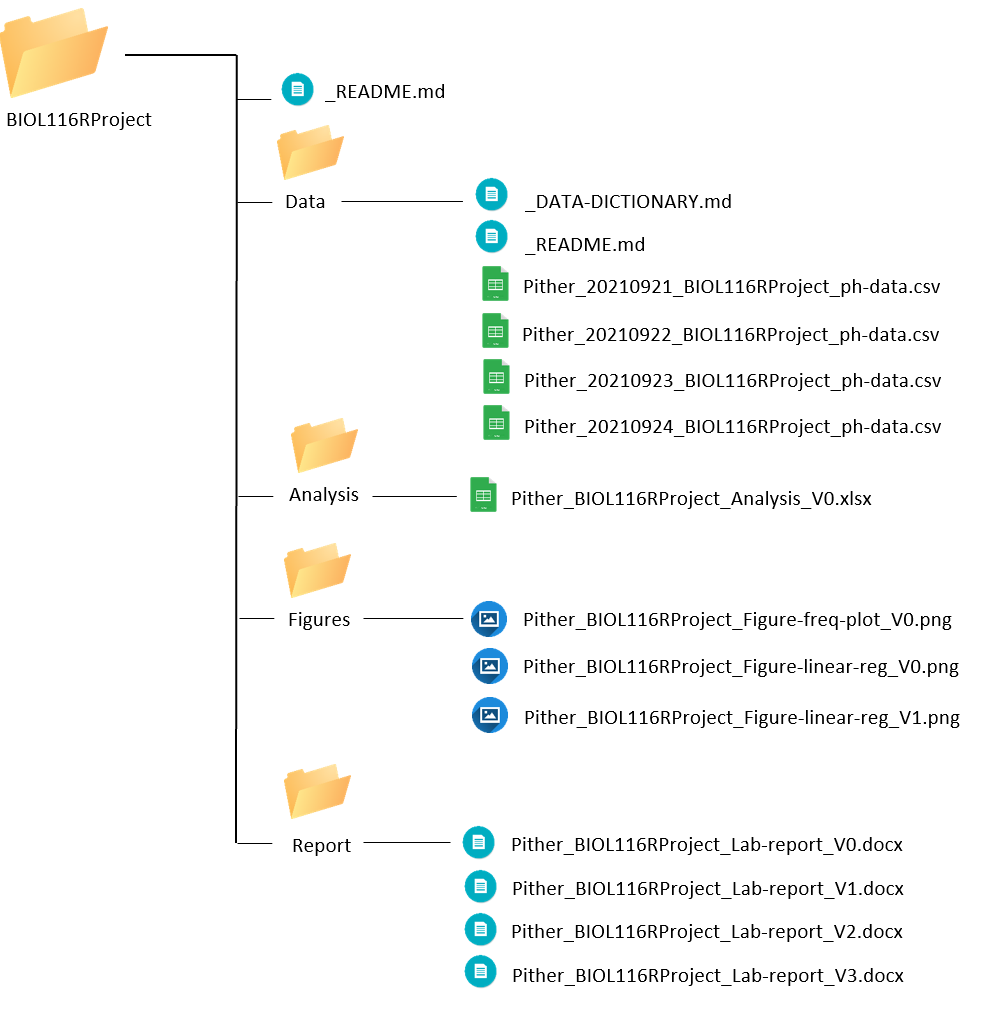
\includegraphics{images/DS_biol116-directory-example.png}

\hypertarget{example-biol-125}{%
\section{Example BIOL 125}\label{example-biol-125}}

Let's work through another example where we start our project off using both appropriate directory structure and file naming conventions. Say you're a student in BIOL 125 working on a research project testing mealworm food preferences\ldots{}

\hypertarget{day-1-1}{%
\subsection*{Day 1}\label{day-1-1}}
\addcontentsline{toc}{subsection}{Day 1}

On day one of our research project, we are asked to prepare the beginning of a lab report that states our research question, hypothesis, and proposed methods. First, we need to create the root folder for our project:

\begin{verbatim}
BIOL125MealwormProject/
\end{verbatim}

Within our root folder we create a \_README.md file to describe our directory structure. Let's add our project name, date the folder was created and who created it, a short description of the project, group member names, file structure (major folders and their proposed content), and naming conventions to this readme file. Your file should look something like this:

\href{files/DS_biol-125-readme_V0.md}{\_README.md}

Since we have just started our project, there won't be files in most subfolders we create. However, it's good to have the skeleton of what we want our directory to look like so everyone in the group places new files in the correct location. Later, if needed, we can modify our directory structure and update our readme file to reflect those changes.

Since we will be using the naming conventions outlined in Chapter 1, we can list those naming conventions here. It may seem strange to outline the naming conventions for documents that haven't been created yet, but having a strategy for naming files from the beginning of the project is very important. It ensures everyone is following the same set of rules when they add or edit files in the project, which helps everyone stay on the same page when working in a shared directory.

Now that our root folder and root readme files are set up, we need to create the subfolders within BIOL125MealwormProject/. Since we outlined the major subfolders in our readme file as Report, Data, Analysis, and Figures, we'll use these same names when we create the subfolders. Finally, we can open up a new Word document for our lab report and save it to the Report folder using the appropriate naming conventions.

\begin{verbatim}
Pither_BIOL125MealwormProject_report_V0.docx
\end{verbatim}

Here is what our project directory looks like so far:

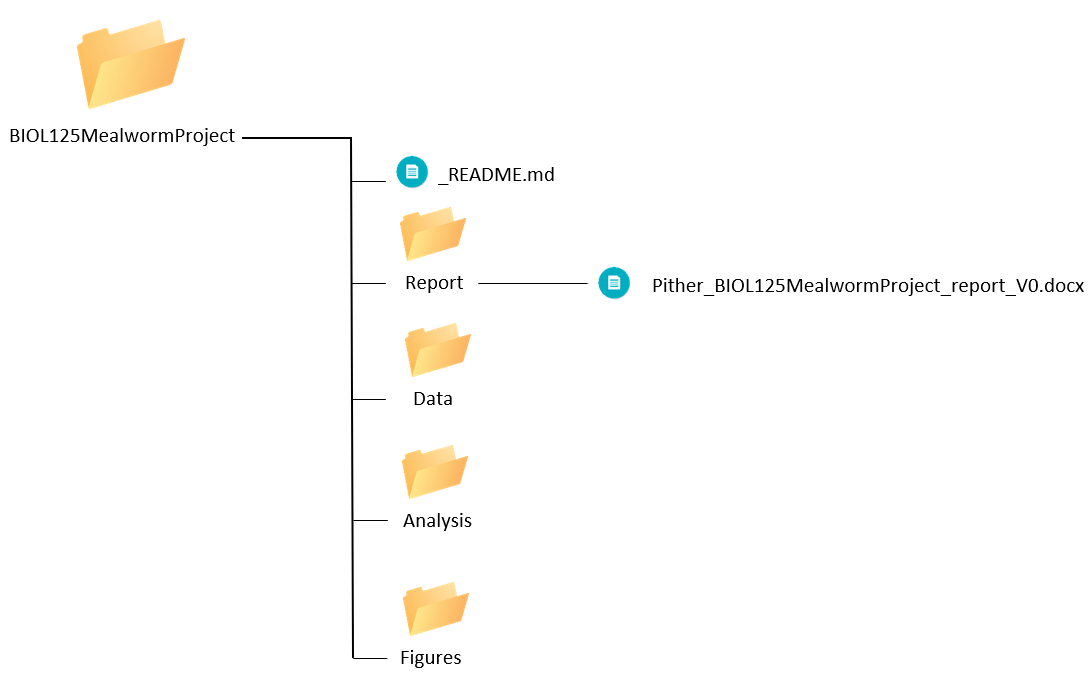
\includegraphics{images/DS_directory-example-1.png}

\hypertarget{day-2-1}{%
\subsection*{Day 2}\label{day-2-1}}
\addcontentsline{toc}{subsection}{Day 2}

Today, we completed a pilot experiment and collected some data. We saved this data file into our project's corresponding Data folder using appropriate naming conventions.

New files:

\begin{verbatim}
Pither_20210915_BIOL125MealwormProject_food-preference-data.csv
\end{verbatim}

Since we have added our first dataset into our project folder, we need to create a corresponding data directory \_README.md and \_DATA-DICTIONMARY.md.

Let's start by creating the data directory readme and provide a description of our data set, collection methods, who collected the data, and where it was collected. It should look something like this:

\href{files/DS_biol-125-data-readme_V0.md}{\_README.md}

Next, let's create a data dictionary for our new dataset. It should look something like this:

\href{files/DS_biol-125-data-dictionary_V0.md}{\_DATA-DICTIONARY.md}

Now our project directory looks like this:

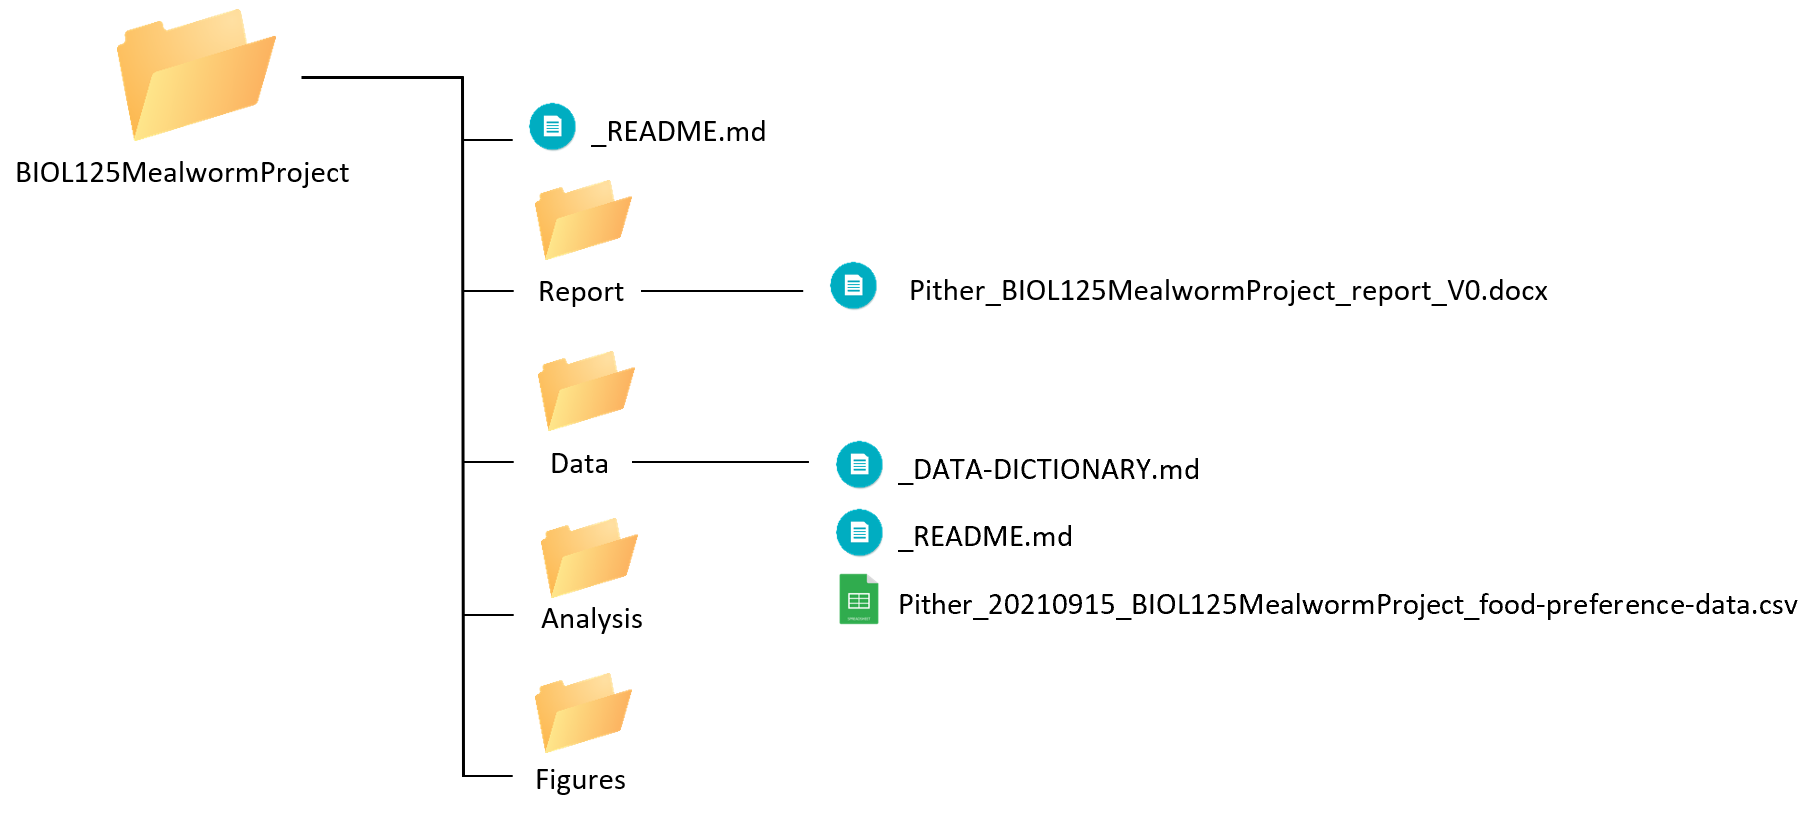
\includegraphics{images/DS_directory-example-2.png}

\hypertarget{day-3}{%
\subsection*{Day 3}\label{day-3}}
\addcontentsline{toc}{subsection}{Day 3}

Now that our group has completed its pilot project, we decided to expand our data collection and start recording how far mealworms are willing to travel to get each food. In addition to this new distance data we continued to collect data on food preferences.

New files:

\begin{verbatim}
Pither_20210916_BIOL125MealwormProject_food-preference-data.csv
Pither_20210916_BIOL125MealwormProject_distance-data.csv
\end{verbatim}

Since we have a new dataset we'll have to update our data directory readme file with a description of the new dataset. Remember to note down the date it was updated and who it was updated by. Our updated data directory \_README.md file should look something like this:

\href{files/DS_biol-125-data-readme_V1.md}{\_README.md}

Now our updated data directory readme file includes descriptions for both datasets.

In the interest of organization, let's keep our food preferences and distance data in their own subfolders. So, we'll create two new subfolders within the Data folder. We'll call one Food-preferences/ and the other Distance/. This way we can organize csv files into the folder for the corresponding dataset. After doing this, we need to update the \_README.md in our root folder, since we've modified our directory structure. This readme should now look something like this:

\href{files/DS_biol-125-readme_V1.md}{\_README.md}

Next, let's also create a data dictionary for our new dataset within our distance subfolder. Remember to note down the date it was updated and who it was updated by. It should look something like this:

\href{files/DS_biol-125-data-dictionary-distance_V0.md}{\_DATA-DICTIONARY.md}

Since we made some updates to our project design and methods, I'll also go ahead and updated our lab report to reflect those changes alongside justification for the changes. Then, I'll be sure to save my updated lab report using the appropriate naming conventions.

\begin{verbatim}
Pither_BIOL125MealwormProject_report_V1.docx
\end{verbatim}

Now our project directory looks like:

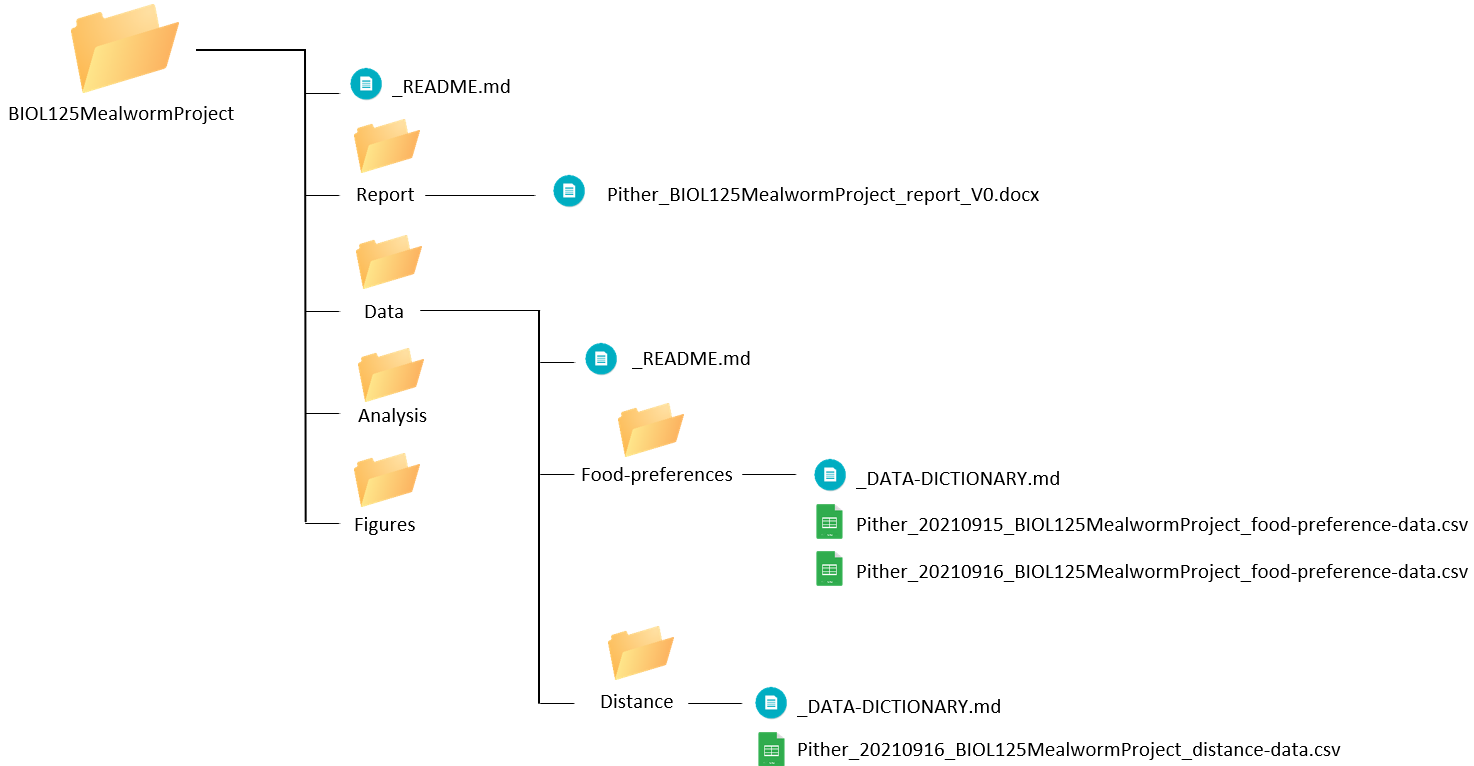
\includegraphics{images/DS_directory-example-3.png}

\hypertarget{day-4-5}{%
\subsection*{Day 4-5}\label{day-4-5}}
\addcontentsline{toc}{subsection}{Day 4-5}

Over these days, we collected our last rounds of data, created some figures, and analyzed the data. So we have a bunch of new files that we need to make sure are placed correctly within our project directory.

New files:

\begin{verbatim}
Pither_20210917_BIOL125MealwormProject_food-preference-data.csv
Pither_20210917_BIOL125MealwormProject_distance-data.csv
Pither_20210918_BIOL125MealwormProject_distance-data.csv
Pither_20210918_BIOL125MealwormProject_Analysis_V0.xlsx
Pither_20210918_BIOL125MealwormProject_Figure-mosaic_V0.png
Pither_20210918_BIOL125MealwormProject_Figure-scatterplot_V0.png
\end{verbatim}

We'll save all 3 new data files into the Data/ subfolder of our directory. Since we've already described these datasets in the data directory \_README.md file and have a corresponding \_DATA-DICTIONARY.md for both, there are no more updates needed.

Next, we'll save our analysis into the Analysis/ subfolder and the figures into the Figure/ subfolder.

Now our project directory looks like:

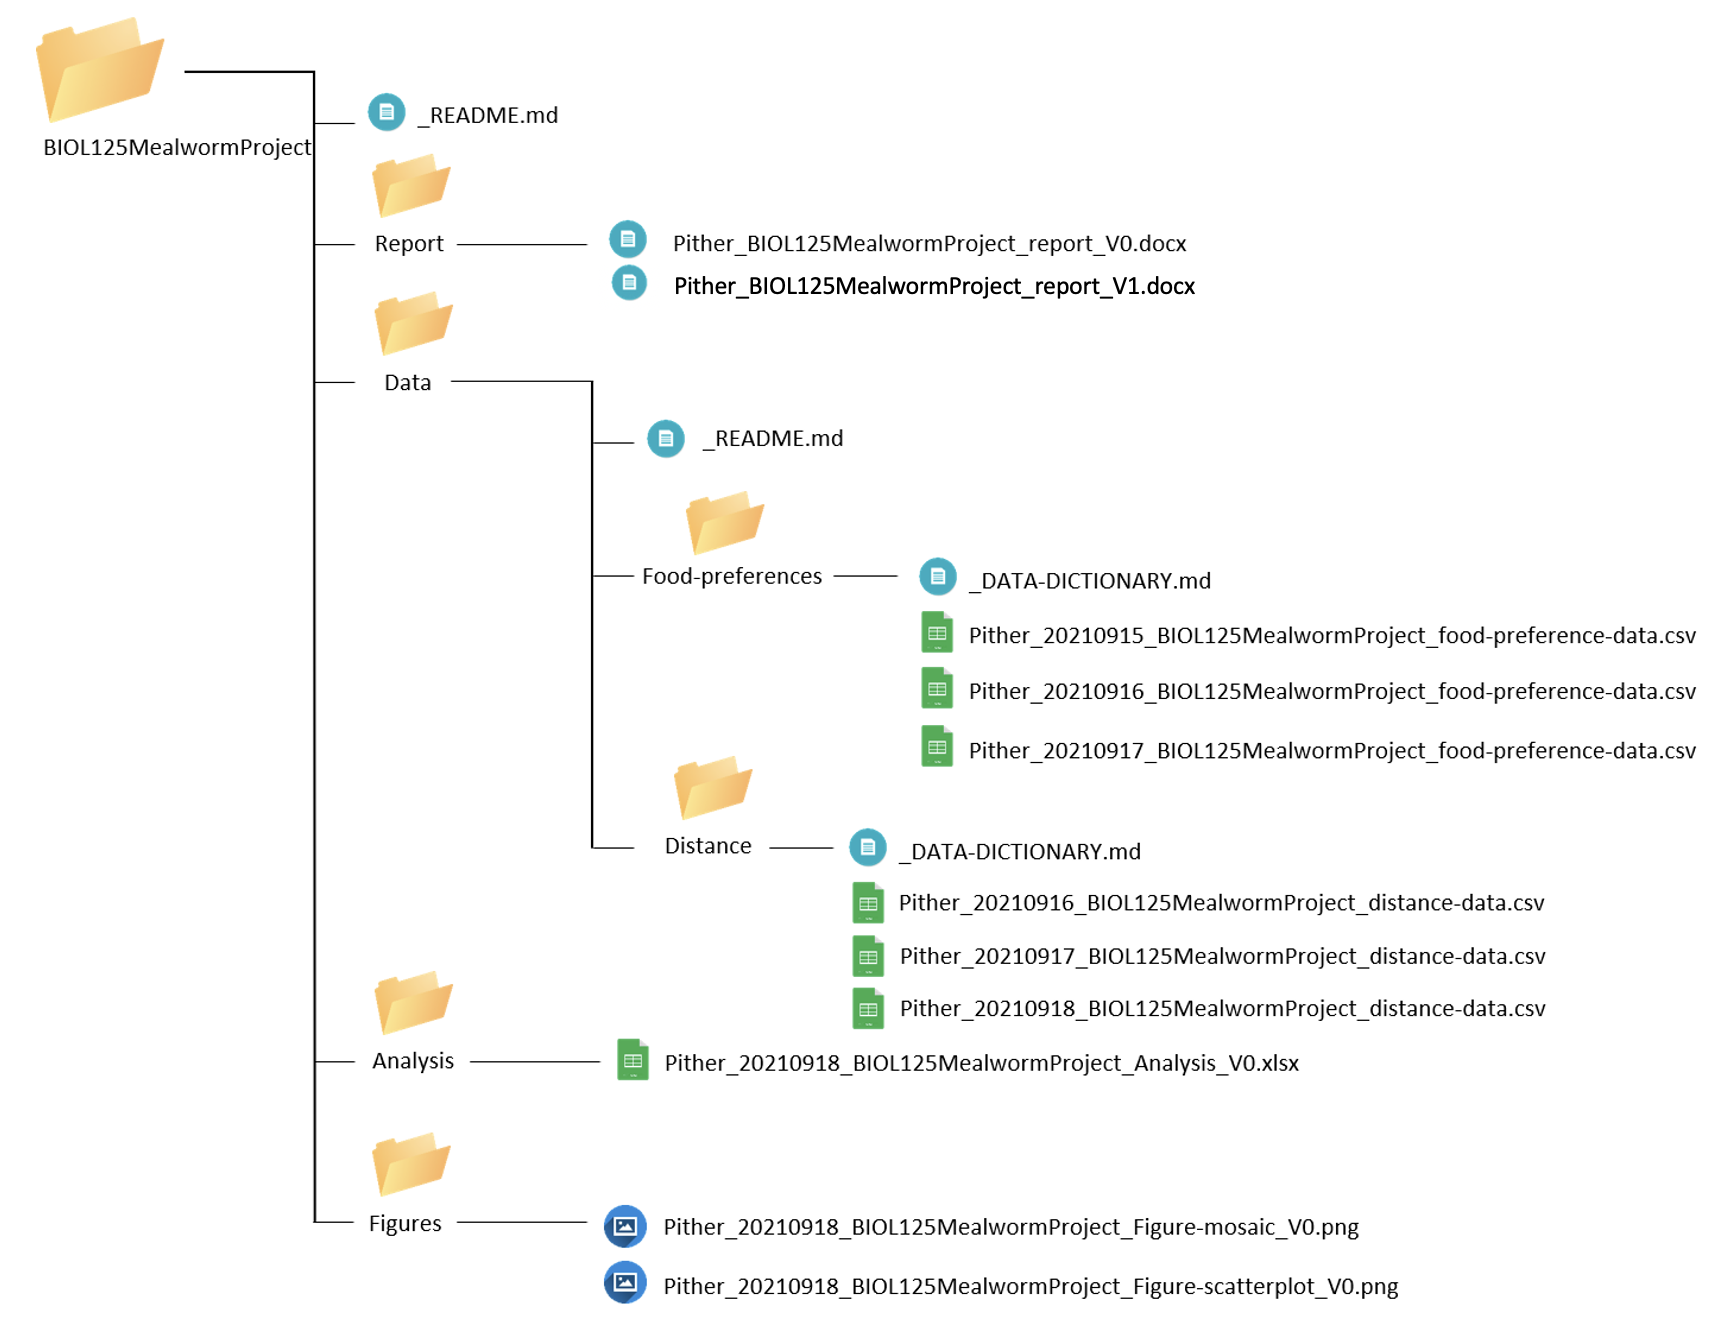
\includegraphics{images/DS_directory-example-4.png}

\hypertarget{day-6-1}{%
\subsection*{Day 6}\label{day-6-1}}
\addcontentsline{toc}{subsection}{Day 6}

Today is the last day of our project and we completed the final copy of our report. We will make sure this is saved into the Report folder using the appropriate naming conventions.

New files:

\begin{verbatim}
Pither_BIOL125MealwormProject_report_V2.docx
\end{verbatim}

Our final directory looks like this:

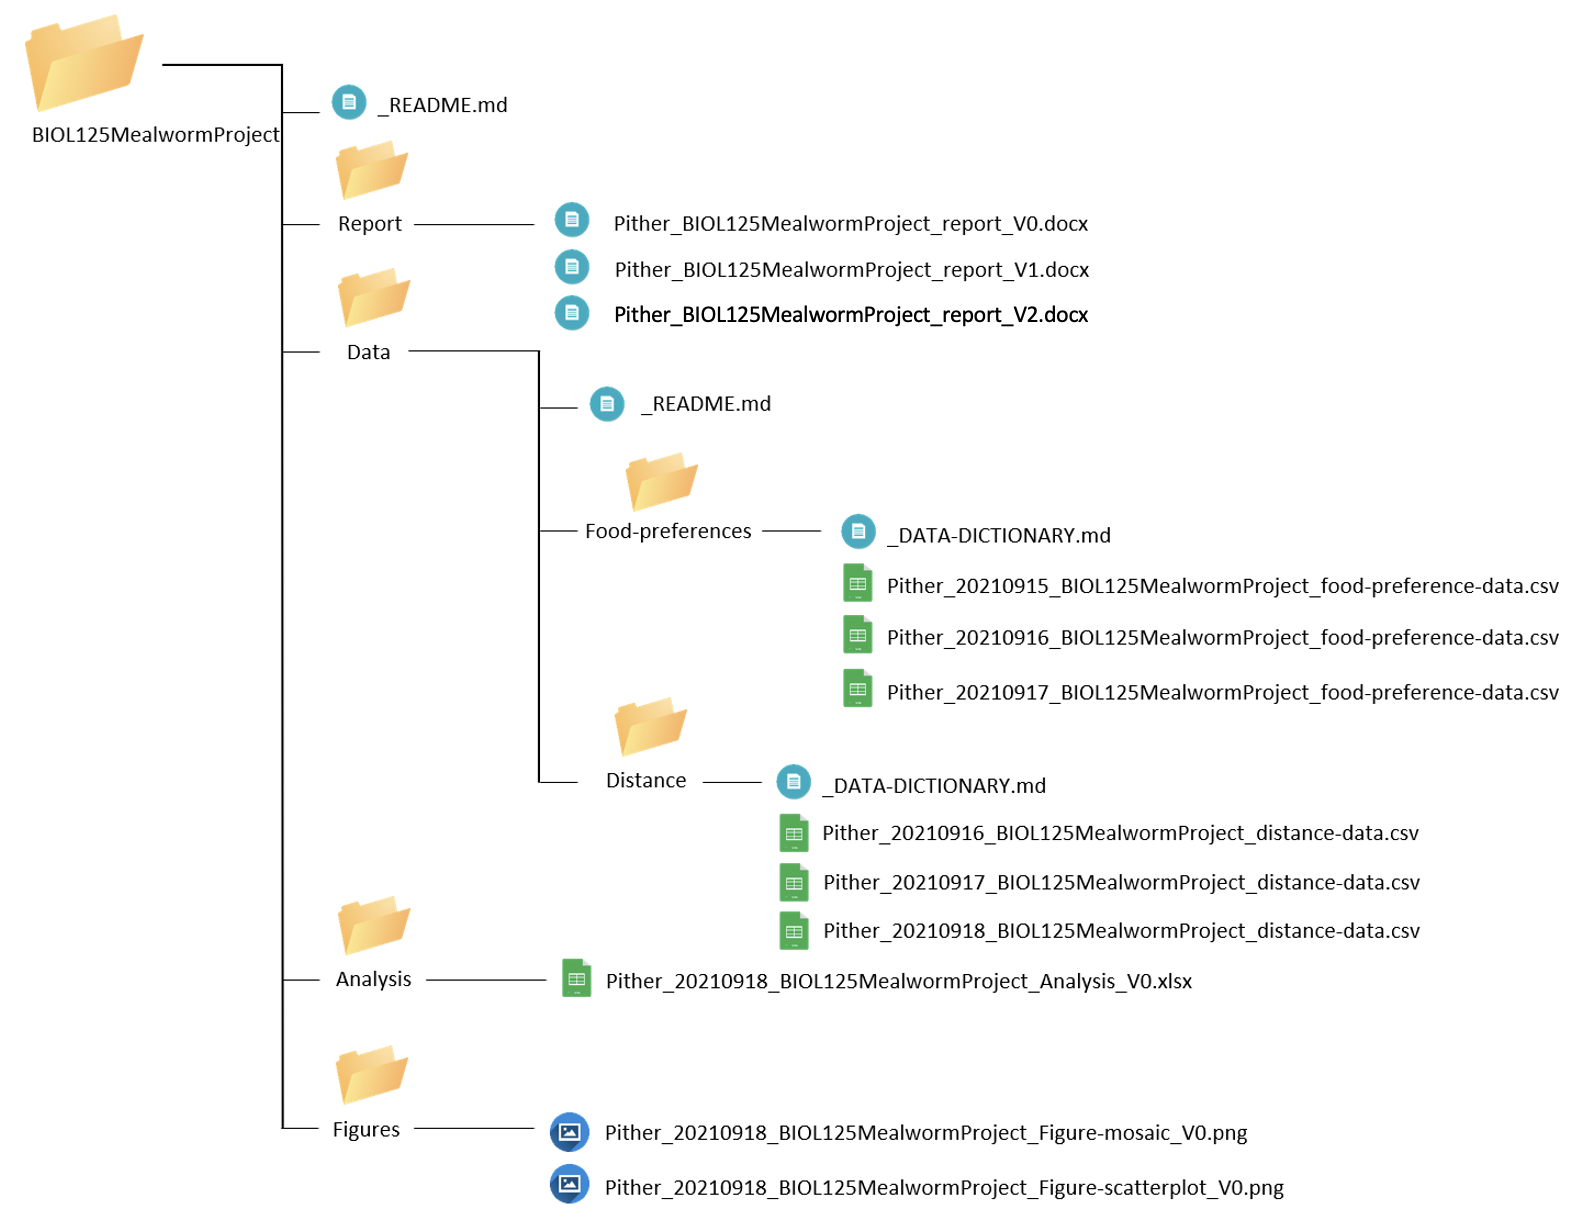
\includegraphics{images/DS_directory-example-5.png}

We can start to see that if you were to share your entire project directory with another person it would be relatively easy for them to locate files and understand the meaning behind each document in our project. They would also know when changes were made and who made these changes, so if they had any questions, they'd know exactly who to ask!

\hypertarget{tidy-data}{%
\chapter{Tidy data}\label{tidy-data}}

We've talked about file naming, directory structures, and documentation to ensure accessible, interpretable, and transparent data. Now it's time to talk about organizing individual variables within a given file. When well organized, data values can be effectively analyzed, summarized, and visualized. When not, they can be onerous to work with and risk misinterpretation.

In general, your data files should adhere to the principles of "tidy data". Tidy data is governed by the following 3 rules\footnote{See: Wickham, H. \& Grolemund, G. (2017). \href{https://r4ds.had.co.nz/tidy-data.html}{Tidy Data}. \emph{In R for Data Science}.}:

\begin{itemize}
\tightlist
\item
  Each variable must have its own column.
\item
  Each observation must have its own row.
\item
  Each value must have its own cell.
\end{itemize}

It's easy to veer from these rules, as it's often easier to collect data using data collection tools that violate these rules. When this is the case, we need to know how to re-organize our data to make it "tidy".

\hypertarget{wide-data}{%
\section{Wide Data}\label{wide-data}}

Non-tidy data - sometimes called "wide" data as it tends to use more columns, but fewer rows - tends to lump observations together in cells. It is often easier to collect data in this way.

So, say we collected data about the number of trout caught at local lakes across several days. We might end up with the following data tables if we used a separate table, sheet of paper etc. to record our findings.

\begin{longtable}[]{@{}ll@{}}
\toprule
Site & Trout\_Caught\_Day\_1 \\
\midrule
\endhead
Mabel-lake & 1 \\
Postill-lake & 3 \\
Ellison-lake & 0 \\
\bottomrule
\end{longtable}

\begin{longtable}[]{@{}ll@{}}
\toprule
Site & Trout\_Caught\_Day\_2 \\
\midrule
\endhead
Mabel-lake & 1 \\
Postill-lake & 3 \\
Ellison-lake & 0 \\
\bottomrule
\end{longtable}

\begin{longtable}[]{@{}ll@{}}
\toprule
Site & Trout\_Caught\_Day\_3 \\
\midrule
\endhead
Mabel-lake & 1 \\
Postill-lake & 3 \\
Ellison-lake & 0 \\
\bottomrule
\end{longtable}

It is also very likely though that we set up an Excel sheet where we recorded the site as the first column and our days and fish caught combined in subsequent columns, one column for each day. Even if we hadn't collected our data this way, we might be tempted to group our above data together for analysis or assignment submission in this way.

Doing this, we'd end up with a table something like the following:

\begin{longtable}[]{@{}llll@{}}
\toprule
Site & Trout\_Caught\_Day\_1 & Trout\_Caught\_Day\_2 & Trout\_Caught\_Day\_3 \\
\midrule
\endhead
Mabel-lake & 1 & 3 & 3 \\
Postill-lake & 3 & 4 & 5 \\
Ellison-Lake & 0 & 5 & 1 \\
\bottomrule
\end{longtable}

But for analysis - for "tidy" data - we want one column per variable. In this case, we have three variables:

\begin{itemize}
\tightlist
\item
  site
\item
  day
\item
  quantity caught
\end{itemize}

So let's get this cleaned up\ldots{}

\hypertarget{tidy-data-1}{%
\section{Tidy Data}\label{tidy-data-1}}

In the previous example, our data were organized where day and quantity caught shared common columns. That is, not every variable had a dedicated column and consequently, not every variable had a value in every given cell - day did not have any cell values.

Tidy data breaks this down and reserves on column per variable and one row per observation. Remember, we have three variables: site, day, and quantity caught. So let's transform this\ldots{}

First, working with a collection tool where we have one table per day:

\begin{longtable}[]{@{}lll@{}}
\toprule
Site & Day & Trout\_Caught \\
\midrule
\endhead
Mabel-lake & 1 & 1 \\
Postill-lake & 1 & 3 \\
Ellison-lake & 1 & 0 \\
\bottomrule
\end{longtable}

\begin{longtable}[]{@{}lll@{}}
\toprule
Site & Day & Trout\_Caught \\
\midrule
\endhead
Mabel-lake & 2 & 3 \\
Postill-lake & 2 & 4 \\
Ellison-lake & 2 & 5 \\
\bottomrule
\end{longtable}

\begin{longtable}[]{@{}lll@{}}
\toprule
Site & Day & Trout\_Caught \\
\midrule
\endhead
Mabel-lake & 3 & 3 \\
Postill-lake & 3 & 5 \\
Ellison-lake & 3 & 1 \\
\bottomrule
\end{longtable}

And second, gathering this data into a single dataset, sorted by site:

\begin{longtable}[]{@{}lll@{}}
\toprule
Site & Day & Trout\_Caught \\
\midrule
\endhead
Mabel-lake & 1 & 1 \\
Mabel-lake & 2 & 3 \\
Mabel-lake & 3 & 3 \\
Postill-lake & 1 & 3 \\
Postill-lake & 2 & 4 \\
Postill-lake & 3 & 5 \\
Ellison-lake & 1 & 0 \\
Ellison-lake & 2 & 5 \\
Ellison-lake & 3 & 1 \\
\bottomrule
\end{longtable}

Now that's tidy data!

\hypertarget{side-by-side-comparison}{%
\section{Side by Side Comparison}\label{side-by-side-comparison}}

\hypertarget{wide-data-1}{%
\subsection*{Wide Data}\label{wide-data-1}}
\addcontentsline{toc}{subsection}{Wide Data}

\begin{longtable}[]{@{}llll@{}}
\toprule
Site & Trout\_Caught\_Day\_1 & Trout\_Caught\_Day\_2 & Trout\_Caught\_Day\_3 \\
\midrule
\endhead
Mabel-lake & 1 & 3 & 3 \\
Postill-lake & 3 & 4 & 5 \\
Ellison-Lake & 0 & 5 & 1 \\
\bottomrule
\end{longtable}

\hypertarget{tidy-data-2}{%
\subsection*{Tidy Data}\label{tidy-data-2}}
\addcontentsline{toc}{subsection}{Tidy Data}

\begin{longtable}[]{@{}lll@{}}
\toprule
Site & Day & Trout\_Caught \\
\midrule
\endhead
Mabel-lake & 1 & 1 \\
Mabel-lake & 2 & 3 \\
Mabel-lake & 3 & 3 \\
Postill-lake & 1 & 3 \\
Postill-lake & 2 & 4 \\
Postill-lake & 3 & 5 \\
Ellison-lake & 1 & 0 \\
Ellison-lake & 2 & 5 \\
Ellison-lake & 3 & 1 \\
\bottomrule
\end{longtable}

\hypertarget{part-data-presentation}{%
\part*{Data Presentation}\label{part-data-presentation}}
\addcontentsline{toc}{part}{Data Presentation}

\hypertarget{figures-and-tables}{%
\chapter{Figures and Tables}\label{figures-and-tables}}

These guidelines are based on current "best practices" in Biology. You may encounter small differences when working with data or reading the results of research from other disciplines. They aim to achieve consistency among faculty, instructors, and students in how data are summarized and presented within lab reports and research papers.

\hypertarget{tables}{%
\section{Tables}\label{tables}}

When presenting data in a table keep in mind the following:

\begin{itemize}
\tightlist
\item
  The heading is placed above the table.
\item
  The table should be interpretable as a stand alone object using an informative heading and judicious footnotes
\item
  Sample sizes and units are always included
\item
  Use horizontal lines only; these are often placed above and below headings, and at bottom of table
\end{itemize}

\hypertarget{example}{%
\subsection*{Example}\label{example}}
\addcontentsline{toc}{subsection}{Example}

The following is an example of a properly formatted table

\textbf{Table 1.} Summary of trait measurements made on individuals of \emph{Solidago} ssp. collected within shaded and open habitats in the vicinity of Portland, Oregon.

Trait

Habitat: Shaded (n = 20)

Habitat: Open (n+ = 18)

Mean (sd)

95\% confidence limit

Mean (sd)

95\% confidence limit

Leaf area (cm2)

4.59 (0.974)

4.14, 5.05

4.54 (0.972)

4.24, 5.15

Leaf mass (mg)

2.52 (0.765)

2.15, 2.89

w.62 (0.705)

2.25, 2.99

Root mass (mg)

9.97 (2.754)

8.67, 11.26

9.90 (2.454)

8.37, 11.16

+ data for two individuals misplaced

\hypertarget{descriptive-summary-statistics}{%
\section{Descriptive / summary statistics}\label{descriptive-summary-statistics}}

Here are some general guidelines to follow when displaying descriptive or summary statistics:

\begin{itemize}
\tightlist
\item
  Round numbers to one more digit for measures of centre (e.g.~mean), and 2 more digits for measures of spread (e.g.~sd) than was used in measuring the data

  \begin{itemize}
  \tightlist
  \item
    For detailed guidelines about significant digits, consult the following webpage: \url{https://www.physics.uoguelph.ca/significant-digits-tutorial}
  \end{itemize}
\item
  Units are preceded by a space within text passages:

  \begin{itemize}
  \tightlist
  \item
    e.g.~"Average height was 34.2 cm (± 3.43 SEM)."
  \end{itemize}
\end{itemize}

\textbf{Describing Numerical Variables}

\begin{itemize}
\tightlist
\item
  Report mean with standard deviation, and additionally median with inter-quartile range for variables that exhibit a non-normal frequency distribution (e.g.~is skewed) or that includes outliers
\item
  Parameter estimates (i.e.~mean) should be accompanied by measures of uncertainty, i.e.~the \emph{standard error of the mean} (SEM) or confidence \emph{interval} (notation: lower limit -- upper limit); confidence \emph{limits}: (lower limit, upper limit)
\item
  Confidence intervals are strongly encouraged because they inform about \emph{effect size}
\item
  Measures of uncertainty for an estimate, such as SEM, can be preceded by a ± sign; do not make the common mistake of reporting a ± sign with a standard deviation, as it is not a measure of uncertainty in an estimate
\end{itemize}

\textbf{Describing Categorical Variables}

\begin{itemize}
\tightlist
\item
  Report a frequency table (raw data) or a summary table with proportions for categories (the main descriptive statistic of interest), along with the confidence interval for the proportion if appropriate
\end{itemize}

\hypertarget{example-1}{%
\subsection*{Example}\label{example-1}}
\addcontentsline{toc}{subsection}{Example}

\textbf{Table 2.} Descriptive statistics for an experiment investigating the effect of different protein diets on growth of chicks since birth. Chicks were weighed at birth and every second day after that until day 20. For more information on this dataset click \href{https://www.rdocumentation.org/packages/datasets/versions/3.6.2/topics/ChickWeight}{here.}

\begin{longtable}[]{@{}lllll@{}}
\toprule
Variable & n & \% & Mean & SD \\
\midrule
\endhead
Diet 1 Diet 2 Diet 3 Diet 4 & 220 120 120 118 & 38.1 20.8 20.8 20.4 & & \\
Weight (gm) & 578 & & 121.8 & 71.10 \\
Time (days) & 578 & & 10.7 & 6.76 \\
\bottomrule
\end{longtable}

\hypertarget{results-of-statistical-tests}{%
\section{Results of Statistical Tests}\label{results-of-statistical-tests}}

Here are some guidelines for reporting the results of statistical tests:

\begin{itemize}
\tightlist
\item
  Your \emph{Methods} section should clearly state the significance level (α), and this should be decided prior to the study
\item
  Test statistics (e.g.~Student's \emph{t} or an "F" from ANOVA) should be rounded to 2 decimal places, and associated \emph{P}-values should report 3 decimal places, or if smaller than 0.001, then \textless0.001. \emph{P}-values do not indicate effect size, so reporting \emph{P} = 10\^{}-6 is not more impressive than \emph{P} \textless0.001
\item
  Concluding statements should, in the absence of a table, include the test, test statistic value, degrees of freedom (\emph{df}) or sample sizes, \emph{P}-value, and confidence interval (if appropriate) in parentheses.

  \begin{itemize}
  \tightlist
  \item
    For example: "On average, hair loss was significantly greater among fathers compared to childless men (Welch's 2-sample \emph{t}-test; \emph{t} = 4.23; \emph{n} F = 18, \emph{n} C = 20; \emph{P} = 0.018; 95\% CI for difference: 9.34 -- 18.22\%)."\\
  \end{itemize}
\item
  Regression and ANOVA results should be shown in a standard ANOVA table format
\end{itemize}

\textbf{Example of ANOVA table format}

\textbf{Table 3.}

\begin{longtable}[]{@{}llllll@{}}
\toprule
& SS & df & MS & F & P \\
\midrule
\endhead
Treatment & 7.224 & 2 & 3.6122 & 7.29 & 0.004 \\
Error & 9.415 & 19 & 0.4955 & & \\
Total & 16.640 & 21 & 4.1078 & & \\
\bottomrule
\end{longtable}

\hypertarget{figures}{%
\section{Figures}\label{figures}}

When displaying data using a figure, follow these guidelines:

\begin{itemize}
\tightlist
\item
  The figure heading should be placed below the graph and should provide sufficient information so the figure can be interpreted on its own
\item
  The heading can include statistical statements (Fig. 1) or simply describe what is being shown (Fig. 2)
\item
  Sample size(s) must be reported
\item
  The first time a particular type of graph is shown (e.g.~boxplot), details of graph features must be provided. Subsequent figures of the same type can refer to the first for details. See Fig. 2 for an example
\item
  Use hollow symbols so that overlapping points can be seen (Fig. 3)
\item
  Orient all text horizontal (except \emph{y}-axis label), including all tick labels
\item
  Place axis tick marks outside of figure border to avoid overlapping with observations
\item
  Data points should not touch the axes
\item
  Fitted lines (e.g.~least-squares regression) included in figures should be fully explained in the heading,

  \begin{itemize}
  \tightlist
  \item
    e.g.~``Line represents a least-squares linear regression line, \emph{y} = 0.3 + 4.5\emph{x} (\emph{F} = 5.65, df = 36; P = 0.021)''.
  \end{itemize}
\item
  For more complex statistics (e.g.~lines associated with mixed effects models) refer the reader to the text for details
\item
  Bar plots should \textbf{only} be used to visualize categorical data (e.g.~proportion of students with brown or blue eyes) or counts (number of flies on scat)
\item
  When comparing numerical data among categories or groups (Figs. 1,2) use stripcharts (Fig. 1) when sample sizes are small (i.e.~\textless20) and boxplots otherwise (Fig. 2)
\end{itemize}

\hypertarget{examples}{%
\subsection*{Examples}\label{examples}}
\addcontentsline{toc}{subsection}{Examples}

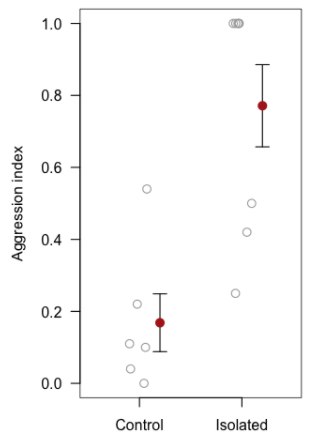
\includegraphics{images/FT_fig-1.png}

\textbf{Figure 1.} Aggression was significantly higher among isolated ants (\emph{n} = 8) compared to the control group (\emph{n} = 6) (see text for details). Shown are individual observations (grey circles), group means (solid circles) with +/- 1 SEM.

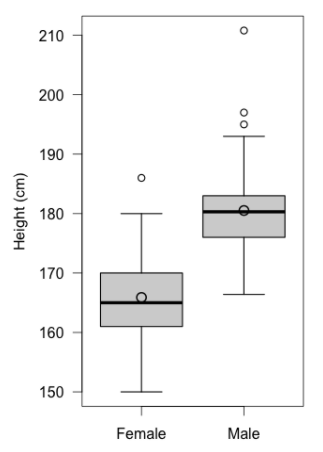
\includegraphics{images/FT_fig-2.png}

\textbf{Figure 2.} Height of male (\emph{n} = 64) and female (\emph{n} = 90) students within BIOL202. Thick horizontal lines represent group medians, large circles represent group means, boxes delimit 1st to 3rd quartiles, whiskers extend to 1.5 x IQR, and small circles represent extreme observations.

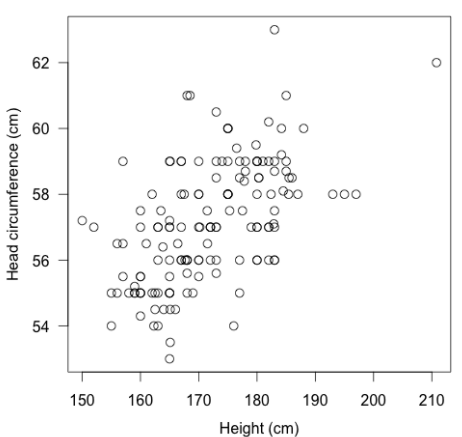
\includegraphics{images/FT_fig-3.png}

\textbf{Figure 3}. Head circumference versus height for \emph{n} = 150 BIOL202 students. The positive association is highly significant (Pearson \emph{r} = 0.82; \emph{P} \textless{} 0.001).

\hypertarget{part-glossary}{%
\part*{Glossary}\label{part-glossary}}
\addcontentsline{toc}{part}{Glossary}

\hypertarget{glossary}{%
\chapter{Glossary}\label{glossary}}

\hypertarget{a}{%
\subsection*{A}\label{a}}
\addcontentsline{toc}{subsection}{A}

\textbf{A priori hypothesis:} Hypothesis that is generated before the research study takes place. Presenting the hypothesis before the study takes place helps in avoiding replacing the hypothesis later with one that fits the data better aka hypothesizing after the fact (HARKing).

\hypertarget{b}{%
\subsection*{B}\label{b}}
\addcontentsline{toc}{subsection}{B}

\textbf{Bias:} Error is introduced and false conclusions might be drawn because our sample doesn't meet established standards for faithful representation of our population of interest.

\textbf{Burden of proof:} The obligation that when a causal link is suggested that evidence to support this link must be presented. This can be accomplished through independent replication of studies where if they demonstrate the same conclusions it reinforces the validity of the causal link between those variables.

\hypertarget{c}{%
\subsection*{C}\label{c}}
\addcontentsline{toc}{subsection}{C}

\textbf{Clinical trials:} Experiments that involve i) human participants who are assigned in advance to a group that receives a particular treatment designed to produce a biomedical or behavioural result and ii) evaluation of the effect of the treatments (NIH, 2017)

\textbf{Citizen science:} When members of the public engage in the research process. Often involving collaboration with researchers.

\textbf{Confirmatory research:} Researchers used a well designed experiment to test the validity of predetermined hypotheses that can be disproved.

\textbf{Critical analysis:} Careful examination and evaluation of all parts of a research article including consideration of the study's strengths and weaknesses as they relate to study design, implementation, data collection, data analysis, and interpretation.

\hypertarget{d}{%
\subsection*{D}\label{d}}
\addcontentsline{toc}{subsection}{D}

\textbf{Descriptive statistics:} A number used to summarize or describe a given data set or sample. Examples include mean, median, mode, standard deviation, and interquartile range.

\textbf{Diversity:} The practice or quality of having individuals who vary in terms of social class, ethnic background, sexual orientation, gender, religion, ability, etc.

\hypertarget{e}{%
\subsection*{E}\label{e}}
\addcontentsline{toc}{subsection}{E}

\textbf{Effect size:} A measure of the degree of association between one variable and another, or in experimental contexts, of the impact of one variable on another.

\textbf{Equity:} The practice of treating all segments of society in such a manner that everyone has a similar chance of achieving a given outcome. Some individuals and groups may need more or different support than others to achieve that outcome. ``Equality'' , in contrast, refers to the practice of providing identical support and opportunities to all.

\textbf{Exploratory research:} Research that is performed to gain a better understanding of an existing problem. For example, it might give rise to hypotheses that can then be tested through confirmatory research.

\hypertarget{f}{%
\subsection*{F}\label{f}}
\addcontentsline{toc}{subsection}{F}

\textbf{File and data management:} Refers to practices used to collect, generate, and store data and files throughout the research process. Researchers should document what type of data they have collected, the methods used, and any relevant context. Files and data should be stored such that they are organized, accessible, and interpretable by both the researcher and others.

\textbf{HARKing:} A form of questionable research practices where the researcher changes their hypothesis after the study is conducted so that the hypothesis better fits the data. In other words, the researcher suggests that this post hoc (after the fact) hypothesis was formed a priori. This has a number of implications including: ``harming the progress of science by preventing the research community from identifying already falsified hypotheses, contributes to the replication crisis, and it increases the probability that the findings are not reproducible or generalizable in the population of interest''. (\href{https://health.ucdavis.edu/ctsc/area/Resource_Library/documents/HARKing_0Jan2021.pdf}{UCDavis Health, n.d.})

\textbf{Hypothesis:} A proposed explanation for an observed phenomenon. Often structured in an ``If\ldots{} then\ldots{} because\ldots{}'' format. Hypotheses must be present a priori, be falsifiable, and measurable.

\textbf{Hypothesis testing:} Typically involves setting a null and alternative hypothesis and performing an appropriate statistical analysis to test those hypotheses. Often used in confirmatory research.

\textbf{Inclusion:} The philosophy or practice of considering individuals from diverse backgrounds in relation to the community, organization, or society, and ensuring that they feel that they belong, supporting them in giving their best efforts, and giving them equal opportunities to advance and participate in decision-making.

\textbf{Literature review:} A review of scholarly sources related to a specific research question or topic. Involves recording a list of research studies consulted, how they were found, and the strengths, limitations, and weaknesses of each.

\textbf{Metadata:} Data that provides information about other data.

\textbf{Open notebooks:} Involves i) publishing or linking to data on an online platform before results are published in a peer-reviewed journal; ii) making information about the methodology and equipment used in a study publicly available; iii) openly discussing both positive and negative results in real time, as they are obtained.

\textbf{Open science:} A movement and set of practices intended to combat the replication crisis, QRPs, and style trumping substance by making all parts of the scientific research process transparent and accessible, allowing for a critical review of how a study was conducted, ultimately enabling that study to be independently replicated. It also involves changing scientific culture to reward not just novel findings, but also the many other aspects of conducting good scientific research.

\textbf{Participatory research:} Turns the relationship between researcher and subject into a partnership, where both contribute to the research question, methods, and outcomes.

\textbf{Peer review:} Peers of the author critically review the author's study. Traditionally peer review focused on the evaluation of studies prior to publication, however open science practices suggest additional peer review at the study design stage prior to implementation. This ensures the study design meets accepted quality standards before it is conducted.

\textbf{Questionable research practices:} A grey area of scientific practice in which researchers do not engage in outright misconduct such as fraud or plagiarism, but may unwittingly break rules of acceptable scientific practice in the pursuit of novel and promising results.

\textbf{R:} a programming language and free software for statistical computing. When used throughout the research process, it allows for openness in the research workflow and computational reproducibility.

\textbf{Replication:} Thorough repetition of a study, using the same methods but different data.

\textbf{Replication crisis}: Many studies cannot be competently analyzed or replicated. This is because critical information about them---design, data, methods, lab notes, analyses and code---may not be made available, or may be poorly communicated. This problem is escalated further because new and original findings are considered more exciting than re-testing or replicating previously conducted studies.

\textbf{Reproducibility:} "Obtaining consistent results using the same input data; computational steps, methods, and code; and conditions of analysis".

\textbf{Research transparency:} The quality or practice of revealing all inputs and outputs of the research process clearly, as well as making evident the exact reasoning and process used in coming to a decision or taking actions in research, in such a way that the study can be replicated. As well, transparency means taking care to disclose important information in a respectful and responsible fashion.

\textbf{Research lifecycle:} The traditional research cycle involves five stages, 1) develop idea, 2) design study, 3) collect and analyze data, 4) write report, and 5) publish report. Traditionally, peer review has been conducted after writing the report and prior to publication. However, open science proposes revising the research life cycle by introducing an additional peer review after the study design stage.

\textbf{Scientific method:} An empirical method for acquiring knowledge which includes making an observation, asking a question, forming a hypothesis, making a prediction based on the hypothesis, and testing the prediction.

\textbf{Scientific integrity:} "The condition resulting from adherence to professional values and practices when conducting, reporting, and applying the results of scientific activities that ensures objectivity, clarity, and reproducibility, and that provides insulation from bias, fabrication, falsification, plagiarism, inappropriate influence, political interference, censorship, and inadequate procedural and information security." (\href{https://www.usda.gov/our-agency/staff-offices/office-chief-scientist-ocs/scientific-integrity-and-research-misconduct}{USDA, n.d.})

\textbf{Statistical analysis:} Involves collecting, organizing, exploring, interpreting, and presenting data to uncover patterns or trends in the data. Involves using statistics to describe the study sample and use that sample to make inferences about the population of interest.

\textbf{Statistical significance:} If a result is determined to have statistical significance it means that the result from the study is not likely to have occurred randomly or by chance. In other words, the result is likely to be caused by something other than chance. The significance level (𝝰) is set by the researcher in advance of the study being performed. Often 𝝰 is set to 0.05, which indicates a 5\% chance of making the wrong decision and determining that the null hypothesis is false when it is in fact true.

\textbf{Study power (aka statistical power):} The probability that a random sample taken from a population will lead to rejection of the study's null hypothesis if that null hypothesis is in fact false. That is, power is a measure of how reliable a study is as a test for its hypothesis; power is positively influenced by things like large sample sizes and relationships characterized by large effect sizes.

\textbf{Version control:} Saving changes to files while retaining the changes on all previous versions of the file. This practice contributes to transparency and openness in science.

\end{document}
